\section{ClojureObject}\label{clojureObject}

ClojureObject

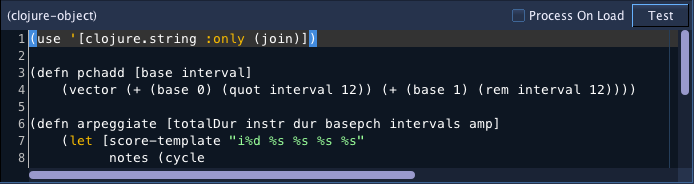
\includegraphics[width=1.00000\textwidth]{images/clojureObject.png}

Accepts NoteProcessors: yes

Allows using the \href{http://www.clojure.org}{Clojure} programming
language to generate score data. The Clojure interpreter is included
with Blue, so ClojureObjects are portable between systems without any
external dependencies. Users do not have to install anything further to
use this object, and the code will continue to function for the duration
of Blue's existence.

When writing your script to generate notes, assign the string value of
the notes to the symbol 'score'. Blue will then read in the value from
that variable and continue processing.

\begin{verbatim}
(def score "i1 0 2 3 4 5")
    
\end{verbatim}

The above example shows the simplest script and will generate a single
note. If the ClojureObject is set with a start time of 0 and a duration
of 2, then it will generate the following score:

\begin{verbatim}
i1  0.0 2   3   4   5
    
\end{verbatim}

\begin{verbatim}
(use '[clojure.string :only (join)])

(defn pchadd [base interval] 
    (vector (+ (base 0) (quot interval 12)) (+ (base 1) (rem interval 12))))

(defn arpeggiate [totalDur instr dur basepch intervals amp]
    (let [score-template "i%d %s %s %s %s"
          notes (cycle 
                    (map #(apply format "%d.%02d" (pchadd basepch %1)) 
                        (concat intervals (subvec intervals 1 (- (count intervals) 1)))))]
    (join \newline
        (map #(format score-template instr %1 dur %2 amp) 
            (range 0 totalDur dur) ; list that will limit the map
            notes))))

(def score (arpeggiate blueDuration 1 0.25 [8 0] [0 4 7] -12))
    
\end{verbatim}

The above example is taken from
blue/examples/soundObjects/clojureSoundObject.blue. This script defines
an apreggiate function, then calls that assigns the value to score.
Notice the use of blueDuration, a symbol that is automatically assigned
to the duration of the ClojureObject.

If the ClojureObject is set with a start time of 0 and a duration of 4,
then it will generate the following score:

\begin{verbatim}
i1  0.0 0.25    8.00    -12
i1  0.25    0.25    8.04    -12
i1  0.5 0.25    8.07    -12
i1  0.75    0.25    8.04    -12
i1  1.0 0.25    8.00    -12
i1  1.25    0.25    8.04    -12
i1  1.5 0.25    8.07    -12
i1  1.75    0.25    8.04    -12
i1  2.0 0.25    8.00    -12
i1  2.25    0.25    8.04    -12
i1  2.5 0.25    8.07    -12
i1  2.75    0.25    8.04    -12
i1  3.0 0.25    8.00    -12
i1  3.25    0.25    8.04    -12
i1  3.5 0.25    8.07    -12
i1  3.75    0.25    8.04    -12
    
\end{verbatim}

Blue processes soundObjects by going through each SoundLayer and
generating score for each object within each layer. This is useful to
know so that if you are using a ClojureObject that has utility functions
that you later use in other ClojureObjects, you should put that utility
ClojureObject on the first SoundLayer closest to the top, or at least on
a layer above all others that contain ClojureObjects.

Also to note, as a feature, Blue uses a single interpreter instance for
processing Clojure code. Therefore, if one ClojureObject has code
evaluated, the values from that code can be read by other objects. This
allows creating utility ClojureObjects. However, one can use stale
values (or values from another project even) if one is not careful to
always assign values in the project that require being set for this
particular project.

The following variables are avaialable from blue:

\begin{description}
\item[blueDuration]
Duration of the Clojure SoundObject
\item[blueProjectDir]
The location of the current project's directory. Includes path separator
at end.
\end{description}

There is a checkbox entitled "Process at Start". Selecting this option
will have the script of the ClojureObject run when a .blue project is
loaded. This is useful for scripts that act as library functions, but
themselves do not generate any notes. For example, you might define a
number of score generation utility functions in one ClojureObject that
has "Process at Start" enabled. Your other ClojureObject may then use
the functions from that ClojureObject Next time you load your project,
if that ClojureObject hasn't been run, your other ClojureObject will not
be able to be run either. If you are rendering from the beginning of a
project, this won't be an issue, but if you're starting work in the
middle of a project, you will need to evaluate that utility
ClojureObject at least once. You can either do a run from the start at
least once, use the "Test" button to have that evaluated, or use
"Process at Start" and have blue ensure it is loaded into the Clojure
interpreter when you load your projects.

Blue is able to load external .clj scripts, resolved from the
.blue/script/clojure or PROJECT\_DIR/script/clojure directory. For
example, if you use:

\begin{verbatim}
(use 'my.script)      
    
\end{verbatim}

This will try to load the script from
"/Users/me/.blue/script/clojure/my/script.clj" or
"/path/to/blueProject/script/clojure/script.clj".
